\documentclass[11pt,aspectratio=169,dvipsnames]{beamer}
\graphicspath{{figs/}}
\usetheme{default}
\usepackage{DasBeamerPaket}
\usepackage{animate}
\usepackage{lastpage}
\usepackage{appendixnumberbeamer}
\usepackage{braket}
\usepackage{booktabs}
\usepackage{tabularx}
\usepackage{tikz}
\setbeamercolor{section in toc}{fg=NavyBlue}
\setbeamercolor{frametitle}{fg=NavyBlue}
\captionsetup[figure]{labelfont=bf}
\captionsetup[table]{labelfont=bf}
\newcommand{\theauthor}{Jakob Krause}
\newcommand{\theshortauthor}{\textsc{J. Krause} for CBELSA/TAPS}
\newcommand{\authormail}{krause@hiskp.uni-bonn.de}
\newcommand{\authorgit}{krausejm}
\newcommand{\thetitle}{Recent Polarization Observable Results in  $\eta$- and $\eta'$-photoproduction off the proton}
\newcommand{\theshorttitle}{$\Sigma$ in $\eta$- and $\eta'$ photoproduction}
\newcommand{\thecolor}{black!70!blue}
\newcommand{\thecolorr}{black!60!blue}
\newcommand{\thecolorrr}{black!50!blue}
\newcommand{\thesubtitle}{Master thesis for the CBELSA/TAPS collaboration}
\newcommand{\thedate}{30th March 2022}
	\makeatletter
\patchcmd{\beamer@calculateheadfoot}{\advance\footheight by 4pt}{\advance\footheight by 20pt}{}{}
\makeatother
\begin{document}
	\definecolor{myWhite}{rgb}{1,1,1}


	\setbeamercolor{coloredboxstuff}{fg=myWhite,bg=\thecolor}
	\setbeamercolor{coloredboxstuff1}{fg=myWhite,bg=\thecolorr}
	\setbeamercolor{coloredboxstuff2}{fg=myWhite,bg=\thecolorrr}	
	\makeatother
	\setbeamertemplate{footline}
	{
		\leavevmode%
		\hbox{%
			\begin{beamercolorbox}[wd=.34\paperwidth,ht=2.25ex,dp=1ex,center]{coloredboxstuff}%
			{\theshortauthor}
			\end{beamercolorbox}%
			\begin{beamercolorbox}[wd=.34\paperwidth,ht=2.25ex,dp=1ex,center]{coloredboxstuff1}%
			{\theshorttitle}
		\end{beamercolorbox}%
			\begin{beamercolorbox}[wd=.34\paperwidth,ht=2.25ex,dp=1ex,center]{coloredboxstuff}%
		\insertframenumber{} / \inserttotalframenumber\hspace*{1ex}
\end{beamercolorbox}}%
	}
	\makeatletter

	
	\setbeamercovered{transparent}
	\setbeamertemplate{navigation symbols}{}
	\setbeamertemplate{frametitle}[default][left,leftskip=0.5cm]
	\setbeamertemplate{itemize item}{\color{black}$\blacktriangleright$}
	\setbeamertemplate{section in toc}[sections numbered]
	\setbeamercolor{section in toc}{fg=\thecolor}
	\setbeamercolor{frametitle}{fg=\thecolor}
	\captionsetup{font=scriptsize,labelfont=scriptsize}
	
	

	
	\begin{frame}[plain]
		\centering
		{\Large \color{\thecolor}{\thetitle}}\\
		\vspace{0.5cm}
		{\thesubtitle}
		\vfill
		\begin{minipage}{\linewidth}
			\centering
			\begin{minipage}{\linewidth}
				\centering
				\textsc{\theauthor}\\
				\scriptsize \href{mailto:\authormail}{\faEnvelope  \hspace*{0.1cm}\authormail} {\color{black}$|$} \href{https://github.com/\authorgit}{\faGithub  \hspace*{0.1cm}\authorgit}\\
			\end{minipage}
			\vspace{.5cm}
			
			{\scriptsize
				Supervisor: \textsc{Jun. Prof. Dr. Annika Thiel}\\
				\tiny \href{mailto:thiel@hiskp.uni-bonn.de}{\faEnvelope  \hspace*{0.1cm}thiel@hiskp.uni-bonn.de}\par}
		\end{minipage}
		\vspace{0.2cm}
		
		\thedate
	\end{frame}


	\begin{frame}{Setting the scene}
			\addtocounter{page}{-1}
		\begin{tcolorbox}[colback=blue!5,colframe=\thecolor,title=The Standard Model of Particle Physics]
			\begin{itemize}
				\item matter consists of 12 (anti-)\emph{fermions}
				\item quarks interact via \emph{strong interaction} 
				\item form bound states: mesons ($q\bar{q}$) and baryons ($qqq$)
			\end{itemize} 
		\end{tcolorbox}
	baryon spectroscopy (photoproduction) gives insight in strong interaction
	\begin{center}
			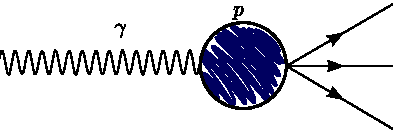
\includegraphics[width=.6\linewidth]{feynman}
	\end{center}


	
	
\end{frame}
\begin{frame}{Setting the scene}
	Observe resonances $R^*$ in the cross sections $\sigma(\gamma p \to R^* \to p M)$
	\vspace{-0.8cm}
	\begin{figure}
		\centering
		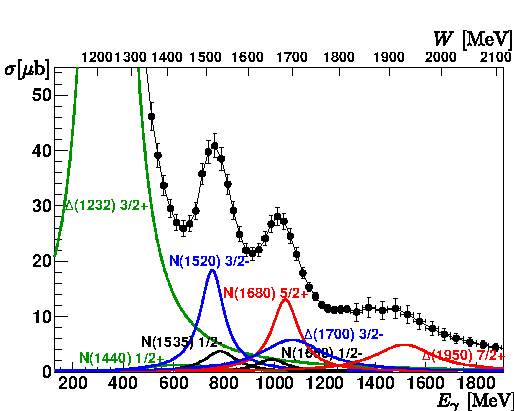
\includegraphics[width=.5\linewidth]{partialwaves}
		\caption*{Total cross section $\sigma(\gamma p \to R^*\to p \pi^0)$ \citef{wuafzth}}
	\end{figure}
$\to$goal: (help to) identify contributing resonances as strong bound states!\\
\end{frame}
\begin{frame}
	\tableofcontents
\end{frame}
\section{Theoretical basics}

\begin{frame}{Theoretical basics}
	\begin{itemize}
		\item resonances are broad, overlapping, require complicated partial-wave-analysis (PWA)
		\item constraints for the analysis can be derived from polarization observables
		\item ultimate goal: "complete experiment"; unambiguous, model-independent PWA solution $\to$ several single and double polarization observables needed
	\end{itemize}
\begin{tcolorbox}[colback=blue!5,colframe=\thecolor,title = Beam-target polarization observables]
\centering
\begin{tabularx}{.7\linewidth}{|l|l|X|X|X|}
	\hline
	\multicolumn{2}{|c}{}&\multicolumn{3}{c|}{\textbf{target polarization}}\\
	\textbf{photon} & &$x$&$y$&$z$\\
	\hline
	unpolarized & $\sigma_0$&-&$T$&-\\
	linearly polarized &\color{red}{$-\Sigma$}&$H$&$-P$&$-G$\\
	circularly polarized &-&$F$&-&$-E$\\
	\hline
\end{tabularx}
\begin{flushright}
	\cites{san}
\end{flushright}
\end{tcolorbox}	
\end{frame}













\begin{frame}{Theoretical basics}



		\begin{tcolorbox}[colback=blue!5,colframe=\thecolor,title=Beam asymmetry $\boldsymbol{\Sigma}$]
			$$\frac{\text{d}\sigma}{\text{d}\Omega}(\varphi)=\frac{\text{d}\sigma}{\text{d}\Omega}_0\left[1-p_\gamma^{\text{lin}}\boldsymbol{\Sigma}\cos(2\varphi)\right]$$
		polarization angle $\varphi$, polarization degree $p_\gamma^{\text{lin}}$
			\begin{flushright}
				{\scriptsize[\cite{san}]}
			\end{flushright}
		\end{tcolorbox}

\begin{figure}
	\centering
	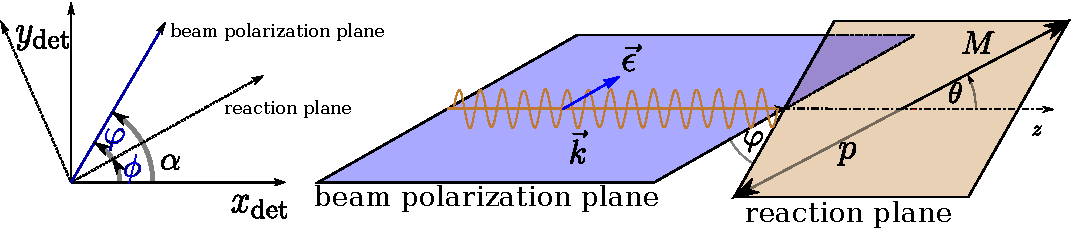
\includegraphics[width=.8\linewidth]{angles.pdf}
	\caption*{Definition of the polarization angle}
\end{figure}
\end{frame}
\section{Experimental Setup}
\begin{frame}{Experimental setup}
	\begin{minipage}{.3\linewidth}
	{\small
			\begin{itemize}
			\item generate photon beam from accelerated electrons via bremsstrahlung, with $E_\gamma\leq\SI{3.2}{\giga\eV}$ 
			\item photon beam impinges on frozen hydrogen target: $\gamma p \to p M\to p X$
			\item measure decay products $X$ of different final states: $M=\pi^0/\eta/\eta'/\dots$
		\end{itemize}
	}
	\end{minipage}
	\begin{minipage}{.69\linewidth}
			\begin{figure}
			\centering
			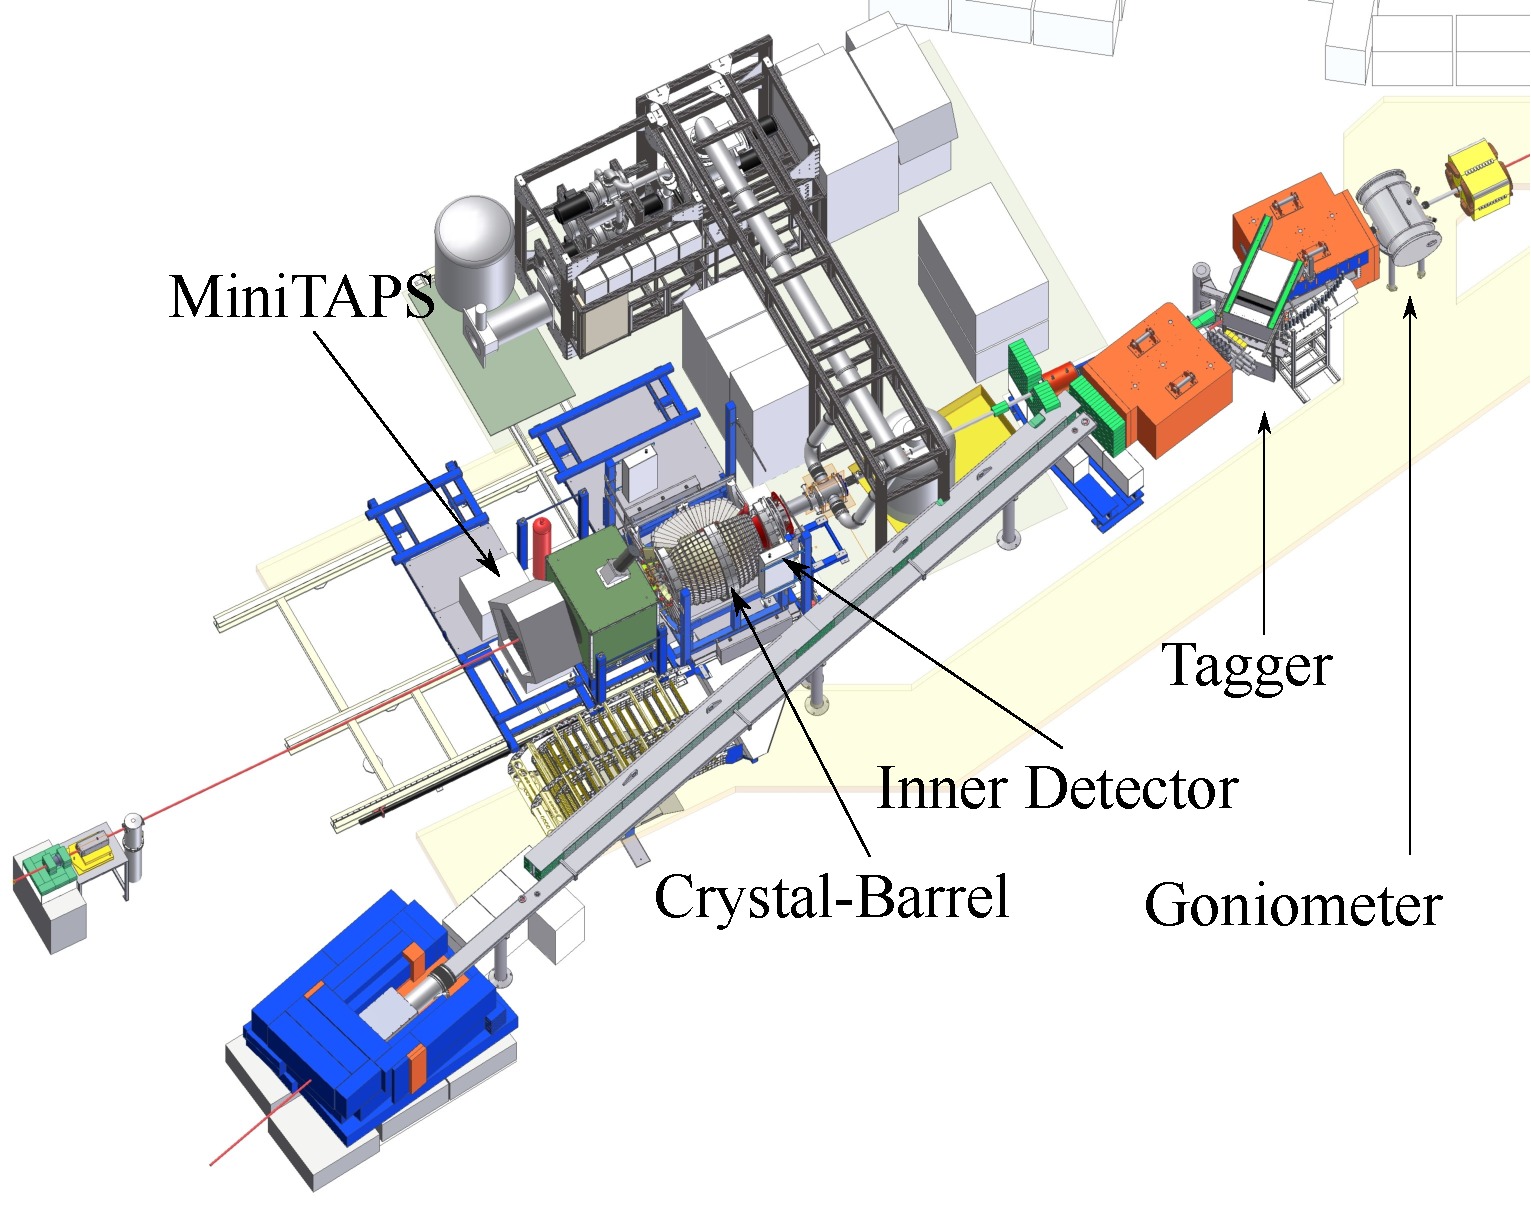
\includegraphics[width=.9\linewidth]{CB-Area}
			\caption*{Overview of the experimental area, adapted from \citef{cb}}
		\end{figure}
	\end{minipage}

\end{frame}

\section{Preliminary results}
\begin{frame}{Event selection ($\eta'$)}


	\begin{minipage}{0.49\linewidth}
	analysis performed in 2x6 bins of $(E_\gamma,\cos\theta_{\eta'}^\text{CMS})$, $E_\gamma\in[1400,1800]$ MeV
	\begin{itemize}
		
		\item 3 detector hits, 2 uncharged, 1 charged
		\item coincident detector hits
		\item kinematic cuts derived from energy-momentum conservation $p_\gamma + p_p = p_p'+p_{\eta'}$
		\item additional cuts to reduce background contributions
	\end{itemize}
total: $\sim 11000$ $\eta'\to\gamma\gamma$ events
		\end{minipage}
	\begin{minipage}{.5\linewidth}
		\begin{figure}
			\centering
			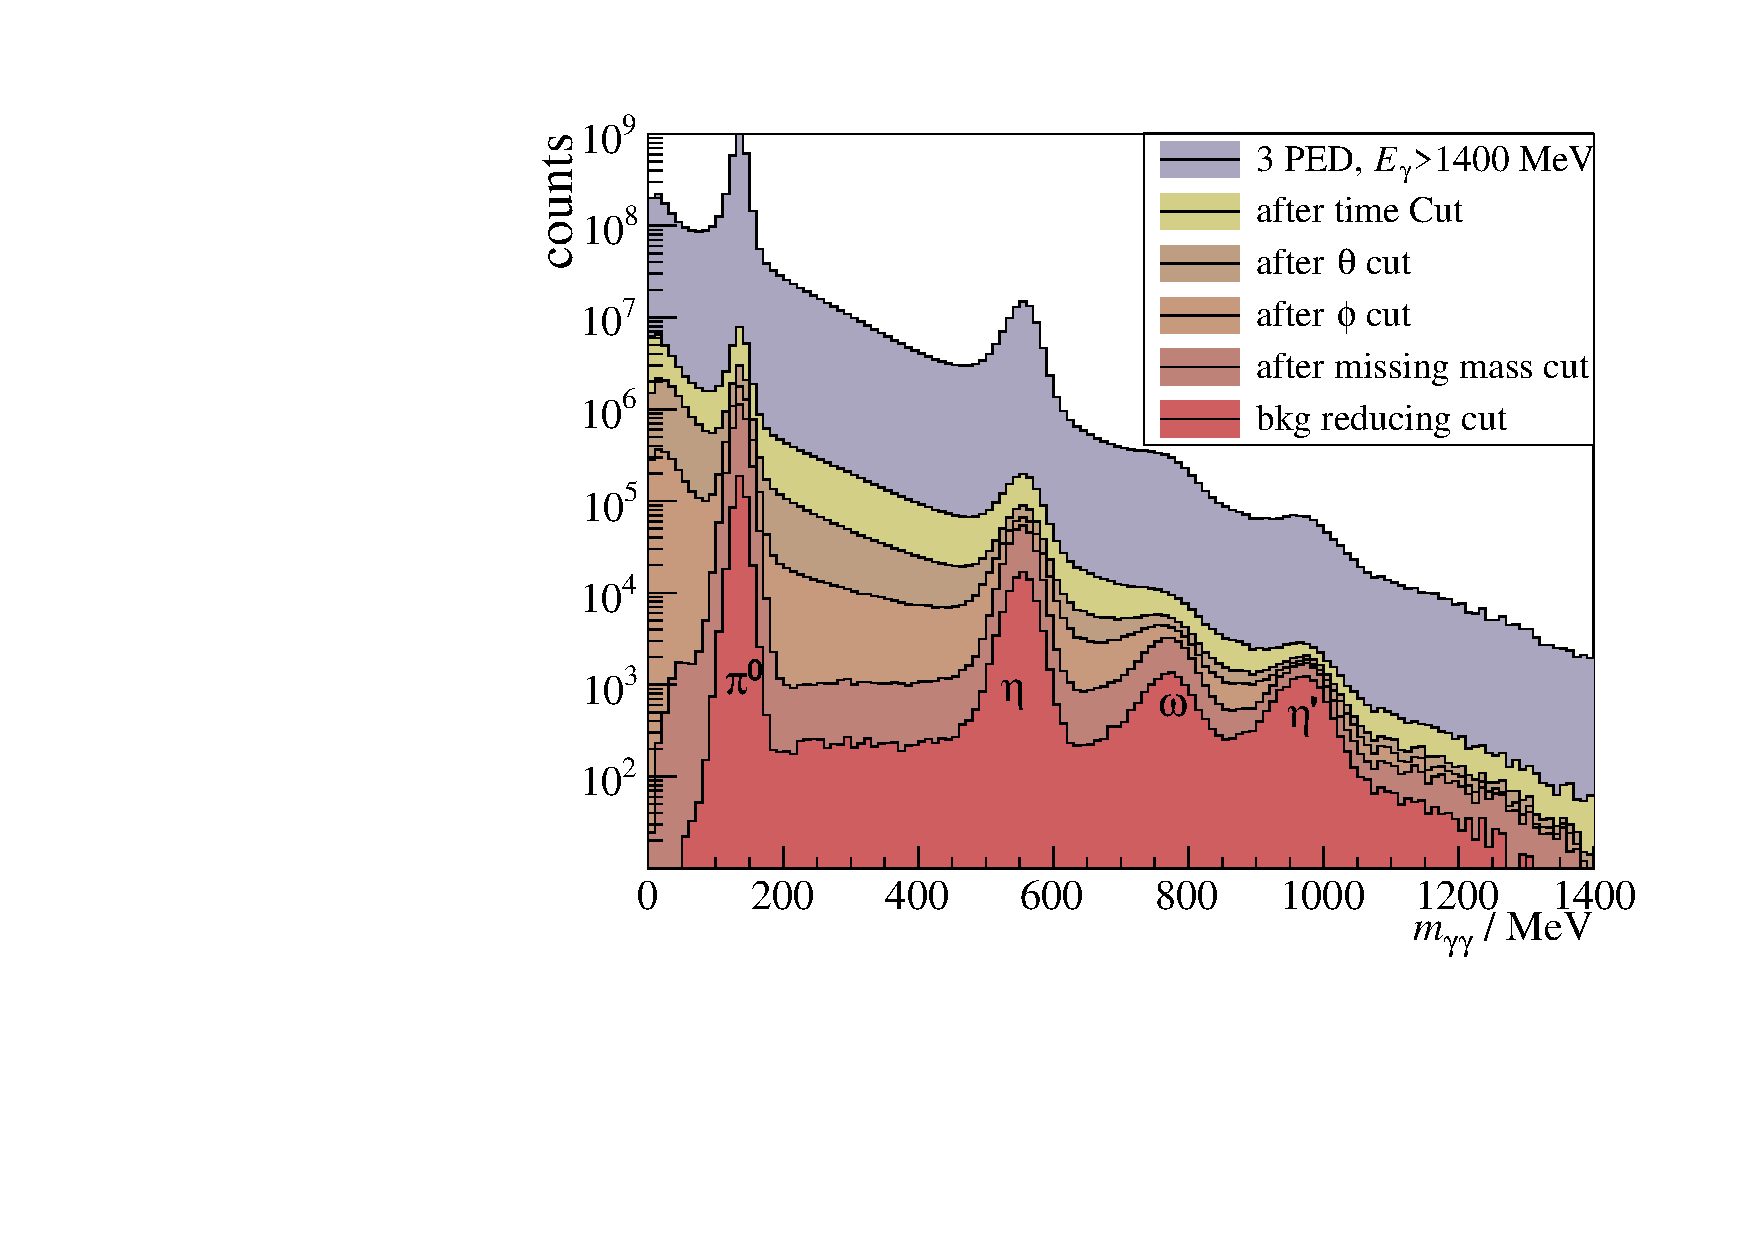
\includegraphics[width=1.05\linewidth]{figs/inv_mass_pretty.pdf}
		\end{figure}
	\end{minipage}




\end{frame}


\begin{frame}{Method ($\eta'$)}

	\begin{itemize}
		\item measure in 2 distinct orthogonal polarization settings $\bot,\parallel$
		\item $\chi^2$-fit to event yield asymmetries $A(E_\gamma,\theta,\phi)=\frac{N^\bot(E_\gamma,\theta,\phi)-N^\parallel(E_\gamma,\theta,\phi)}{p_\gamma^\parallel N^\bot(E_\gamma,\theta,\phi) + p_\gamma^\bot N^\parallel(E_\gamma,\theta,\phi)}=\Sigma(E_\gamma,\theta)\cos\left(2\left(\alpha^\parallel-\phi\right)\right)$
		%\item unbinned fit $\mathcal{L}\propto\prod_i\left[ 1\mp p_{\gamma_i}^{\parallel/\bot}\Sigma\cos\left(2\left(\alpha^\parallel-\phi_i\right)\right)\right]\cdot\epsilon(\phi_i)$
		\item fit from $\sim 800$ $\eta'\to\gamma\gamma$ events
	\end{itemize}
\vspace{-0.5cm}
\begin{figure}
	\centering
	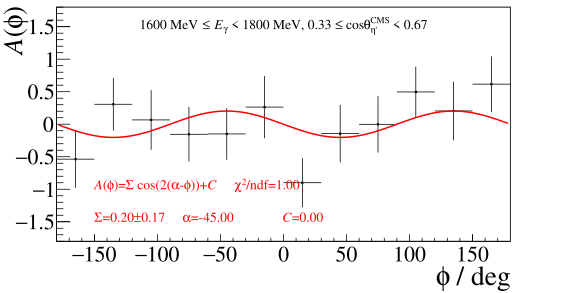
\includegraphics[width=.66\linewidth]{asym_bin}
\end{figure}


\end{frame}
\begin{frame}{Preliminary results ($\eta'$)}
	\begin{figure}
		\centering
		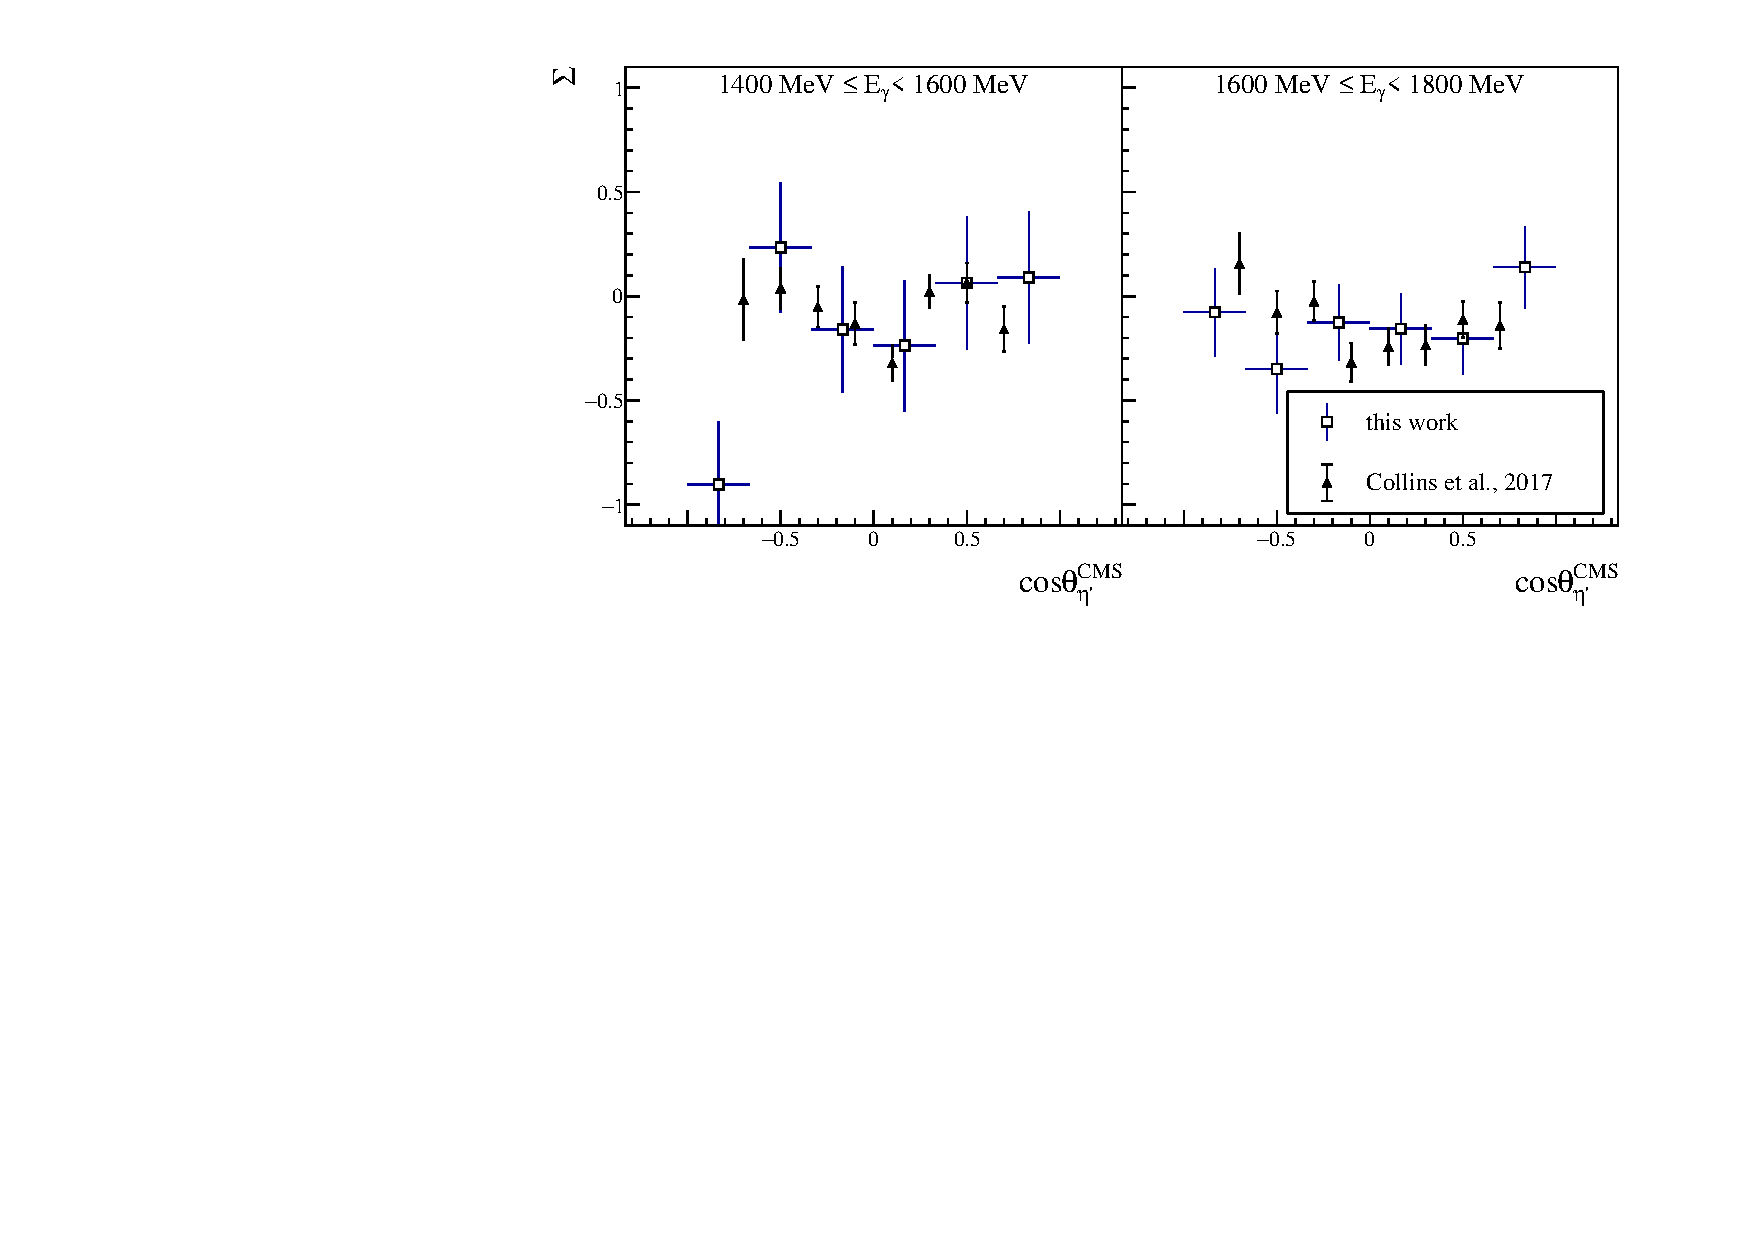
\includegraphics[width=.8\linewidth]{sigma}
		\caption*{Beam asymmetry $\Sigma$ for all energy and angular bins}
	\end{figure}
\end{frame}


\begin{frame}{Preliminary results ($\eta$)}
	\begin{minipage}{\linewidth}
\begin{tcolorbox}[colback=blue!5,colframe=\thecolor,title={Event selection ($\eta$)}]
	analysis performed in 11x12 bins of $(E_\gamma,\cos\theta)$ by \cites{eta}
\end{tcolorbox}
	\end{minipage}
	\begin{minipage}{\linewidth}
\begin{tcolorbox}[colback=blue!5,colframe=\thecolor,title={Method}]
	\begin{itemize}
		\item fit to event yield asymmetries using \textsc{bayesian} inference
		\item $p(\theta|y)\propto\mathcal{L}(\theta,y)\cdot\pi(\theta)$, obtained using \textsc{Markov}-chain-Monte-Carlo (MCMC)
	\end{itemize}
\end{tcolorbox}
	\end{minipage}
	

\end{frame}
\begin{frame}{Preliminary results ($\eta$)}
	\begin{figure}
		\centering
		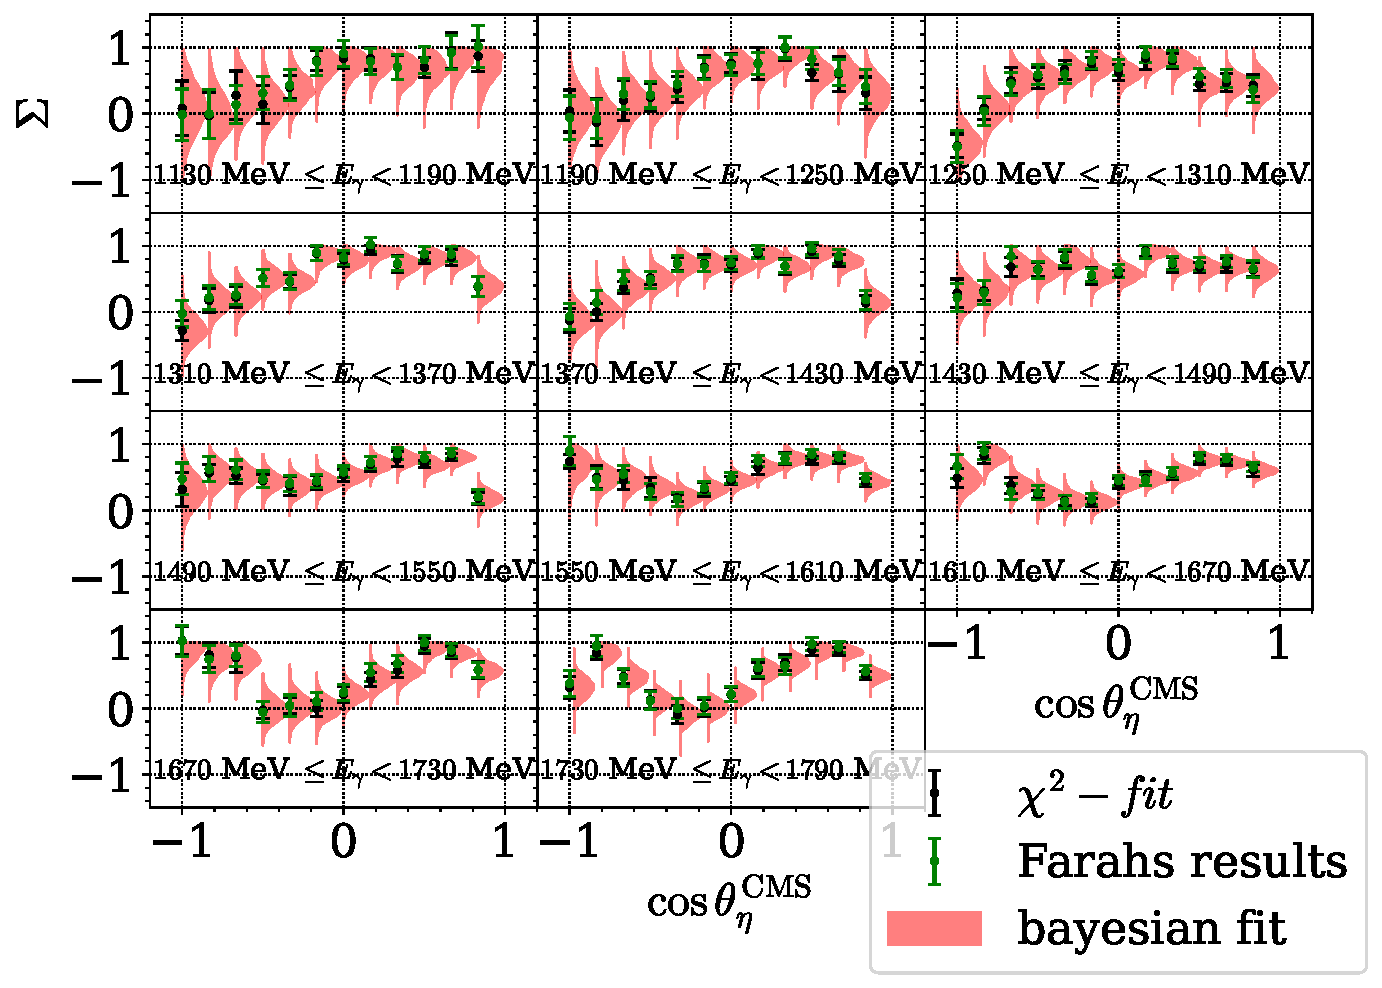
\includegraphics[width=.8\linewidth]{../bayes/realdeal/sigma_eta_alt.pdf}
		\caption*{Beam asymmetry $\Sigma$ for all energy and angle bins}
	\end{figure}
\end{frame}


\section{Conclusion}
\begin{frame}{Conclusion}
	\begin{minipage}{.49\linewidth}
		\begin{tcolorbox}[colback=blue!5,colframe=\thecolor,title={Summary}]
			\begin{itemize}
				\item $\Sigma$ extracted for $\eta$ and $\eta'$ final state
				\item $\eta$ results obtained with \textsc{bayesian} fit agree with previous results 
				\item $\eta'$ results agree with previous results
			\end{itemize}
			\end{tcolorbox}
	\end{minipage}
\begin{minipage}{.49\linewidth}
	\begin{tcolorbox}[colback=blue!5,colframe=\thecolor,title={Outlook}]
		\begin{itemize}
			
			\item extract $\Sigma$ using unbinned maximum likelihood fit for $\eta/\eta'$
			\item apply \textsc{bayesian} approach to above method
			\item consider bkg contaminations in results of $\Sigma_{\eta'}$
			
		\end{itemize}
	\end{tcolorbox}
\end{minipage}
\end{frame}

\appendix
\begin{frame}
	\centering
	\LARGE
	\color{\thecolor}\textsc{Backup \& References}
\end{frame}
\begin{frame}[allowframebreaks]{References}
	    \printbibliography
	
\end{frame}
\begin{frame}{Additional theoretical basics}
	\begin{tcolorbox}[colback=blue!5,colframe=\thecolor,title=Unpolarized differential cross section]
		
		$$\frac{\text{d}\sigma}{\text{d}\Omega}=\frac{1}{4}\rho\sum_{\text{spins}}|\braket{f|\mathcal{F}|i}|^2\\,$$
		where
		$$\mathcal{F}=i(\vec{\sigma}\cdot\vec{\epsilon})F_1+(\vec{\sigma}\cdot\hat{q})(\vec{\sigma}\cdot(\hat{k}\times\vec{\epsilon}))F_2+i(\vec{\sigma}\cdot\hat{k})(\hat{q}\cdot\vec{\epsilon})F_3+i(\vec{\sigma}\cdot\hat{q})(\hat{q}\cdot\vec{\epsilon})F_4$$
		\begin{flushright}
			$F_i:$ complex CGLN Amplitudes
		\end{flushright}
		
		
		\begin{flushright}
			{\scriptsize[\cite{cgln}]}
		\end{flushright}
	\end{tcolorbox}
	$\frac{\text{d}\sigma}{\text{d}\Omega}\in\mathbb{R}$, not sufficient do determine $\mathcal{F}$ unambiguously\\
	$\rightarrow$ Polarization Observables can be related to $F_i$
\end{frame}


\end{document}
